\documentclass[paper=letter, fontsize=11pt]{scrartcl}
\usepackage[dvipsnames]{xcolor}
\usepackage[mathscr]{eucal}
\usepackage{latexsym,amsfonts,amssymb,amsthm,amsmath}
\usepackage{listings,tcolorbox,enumitem,algorithm2e,multirow,framed}
\usepackage{graphicx,float}
\usepackage{geometry}
\geometry{
  top=0.75in,            % <-- you want to adjust this
  bottom=0.75in,
  left=0.75in,
  right=0.75in,
  headheight=3ex,       % <-- and this
  headsep=4ex,          % <-- and this
}
\usepackage{parskip}
%\usepackage{pgfplots}
\usepackage{pdfpages}
\usepackage{mathtools}
\usepackage[T1]{fontenc}
\usepackage{tgtermes}
\usepackage[bb=boondox]{mathalfa}
\usepackage{enumitem}
\usepackage[protrusion=true,expansion=true]{microtype}
\usepackage{url}
%%% Custom sectioning
\usepackage{sectsty}
\allsectionsfont{\centering \normalfont\scshape}
\usepackage{biblatex, hyperref}

%\pgfplotsset{compat=1.16}
\usepackage{fancyhdr}
\renewcommand{\headrulewidth}{0pt}			% Remove header underlines
\renewcommand{\footrulewidth}{0pt}				% Remove footer underlines
\setlength{\headheight}{13.6pt}


%%% Equation and float numbering
\numberwithin{equation}{section}		% Equationnumbering: section.eq#
\numberwithin{figure}{section}			% Figurenumbering: section.fig#
\numberwithin{table}{section}				% Tablenumbering: section.tab#


%%% Maketitle metadata
\newcommand{\horrule}[1]{\rule{\linewidth}{#1}} 	% Horizontal rule

\definecolor{codegreen}{rgb}{0,0.6,0}
\definecolor{codegray}{rgb}{0.5,0.5,0.5}
\definecolor{codepurple}{rgb}{0.58,0,0.82}
\definecolor{backcolour}{RGB}{238,242,245}
\definecolor{mySol}{HTML}{0f3e61}
\definecolor{myPro}{RGB}{29,100,33}

\lstdefinestyle{mystyle}{
    %backgroundcolor=\color{backcolour},   
    commentstyle=\color{codegray},
    keywordstyle=\color{RedOrange},
    numberstyle=\tiny\color{codepurple},
    stringstyle=\color{codegreen},
    basicstyle=\ttfamily\footnotesize,
    breakatwhitespace=false,         
    breaklines=true,                 
    captionpos=b,                    
    keepspaces=true,                 
    numbers=left,                    
    numbersep=5pt,                  
    showspaces=false,                
    showstringspaces=false,
    showtabs=false,                  
    tabsize=2
}
\lstset{style=mystyle}

\theoremstyle{plain}

\newtheorem{theorem*}{Theorem}[section]
\newtheorem{theorem}{Theorem}[section]
\newtheorem{thm}{\textit{Theorem}}
\usepackage{tcolorbox}
\tcbuselibrary{breakable}
\newenvironment{sol}
{
    \renewcommand\qedsymbol{$\blacksquare$}
    \begin{tcolorbox}[
        colback=mySol!10,
        colframe=mySol!10,
        sharp corners,
        breakable
    ]
    \textbf{Solutions:}
}
{
		\begin{flushright}
		\qedsymbol	
		\end{flushright}
    \end{tcolorbox}
}


%      Blackboard bold letters
\newcommand{\set}[2]{\{#1\,:\,\text{#2}\}}
\newcommand{\bR}{\mathbb R}
\newcommand{\bC}{\mathbb C}
\newcommand{\bZ}{\mathbb Z}
\newcommand{\bN}{\mathbb N}
\newcommand{\bQ}{\mathbb Q}
\newcommand{\bF}{\mathbb F}
\newcommand{\ra}{\rightarrow}
\newcommand{\la}{\leftarrow}
\newcommand{\lra}{\leftrightarrows}
\newcommand{\Col}{\mathrm{Col}}
\newcommand{\Row}{\mathrm{Row}}
\newcommand{\tr}{\mathrm{trace}}
\newcommand{\st}{\mathrm{s.t.}}
\newcommand{\abs}[1]{\left| #1 \right|}
\newcommand{\adj}{\operatorname{adj}}
\renewcommand{\vec}[1]{\mathbf{#1}}
\newcommand{\Var}{\mathrm{Var}}
\newcommand{\Cov}{\mathrm{Cov}}
\setcounter{MaxMatrixCols}{20}




	
\addbibresource{reference.bib}
%%% Custom headers/footers (fancyhdr package)
\usepackage{fancyhdr}
\pagestyle{fancyplain}
\fancyhead[R]{\leftmark}
\fancyhead[L]{STAT 443 Project Report}


\title{
		%\vspace{-1in} 	
		\usefont{OT1}{bch}{b}{n}
		\normalfont \normalsize \textsc{{\Large University of Waterloo} \\[0.1cm] 
        Faculty of Mathematics \\[0.1cm] 
        Department of Statistics and Actuarial Science}
  \\ [25pt]
		\horrule{0.5pt} \\[0.4cm]
    		{\huge STAT 443 PROJECT REPORT} \\ [0.3cm]
         {\Large Predicting Monthly Gold Prices (CHF)}
		\horrule{2pt} \\[0.5cm]
}
\author{
		\normalfont 								\normalsize
        Group 2: Xinjie Qiao, Catherine Zhou, Zoe Zou \\[-3pt]		\normalsize
        \today
}
\date{}


\AtBeginDocument{
  \catcode`_=12
  \begingroup\lccode`~=`_
  \lowercase{\endgroup\let~}\sb
  \mathcode`_="8000
}
\let\emptyset\varnothing
\hbadness=99999

\begin{document}

\maketitle
\thispagestyle{empty}

\tableofcontents
\listoftables
\listoffigures


\newpage
\section{Introduction}

Throughout the history and development of economic systems, various goods and materials have
played the role of money. Among them, the most representative one is gold. Even until now, Gold has always been considered a custodian of value and its basic function is to preserve purchasing power in times of great uncertainty. Gold price fluctuation trend prediction is an important issue in the financial world. Even small improvements in predictive performance can make lots of profits.

There are many methods in the literature that make predictions of the price of gold based on
historical data, like random forest \cite{GoldPrice}. For another example, one team also use combines information from NASDAQ index, Hang sen Index to adjust the prediction \cite{PredictionOfGoldPrice}. 


In this project, the topic is to have some naive attempt of prediction of gold price within the scope of STAT 443. The methods that we will use are regression, smoothing methods, and Box-Jenkins models. Moreover, we will evaluate the prediction power by mean square of errors(MSE) and pick the best models.

\vspace{0.2cm}

In this project, our teammates are responsible for the following:

\begin{description}
    \item [Xinjie Qiao] Box-Jenkins models, SARIMA model selection, analysis on the validity of the model
    \item [Catherine Zhou] Extraction of data, power transformation, regression models, project report
    \item [Zoe Zou] Smoothing methods, introduction, presentation slides, presentation recording
\end{description}

\vspace{1cm}
\begin{center}
    \noindent\rule{10cm}{0.4pt}
\end{center}

\section{Analysis}

\subsection{Data}

We find the data from \href{https://www.kaggle.com/datasets/odins0n/monthly-gold-prices?select=1979-2021.csv}{Kaggle}, which contains the monthly gold price per gram from January 1979 to July 2021 from 18 different countries. We choose the Switzerland CHF currency as the data we want to analyze, because the price of the gold includes the fluctuations of the currency exchange rate. In order to make sure that the data only related to the nature volatility of gold price, we decided to choose the currency with more stable exchange rate, in which Switzerland is chosen, as that the country's zero-inflation policy, combined with its political independence, makes CHF an extremely powerful and stable currency \cite{CFI}.

\begin{table}[H]
\centering
\begin{tabular}{|c|c|}
\hline
Date & Switzerland.CHF. \\
\hline\hline
31-01-1979 &  379.3 \\
28-02-1979 &  413.6 \\
30-03-1979   & 406.2 \\
30-04-1979   & 420.0 \\
31-05-1979   & 478.0 \\
29-06-1979   & 457.7 \\
\hline
\end{tabular}
\caption{First 5 rows of the monthly gold price}
\label{table:head}
\end{table}
\vspace{-1cm}
\begin{figure}[H]
    \centering
    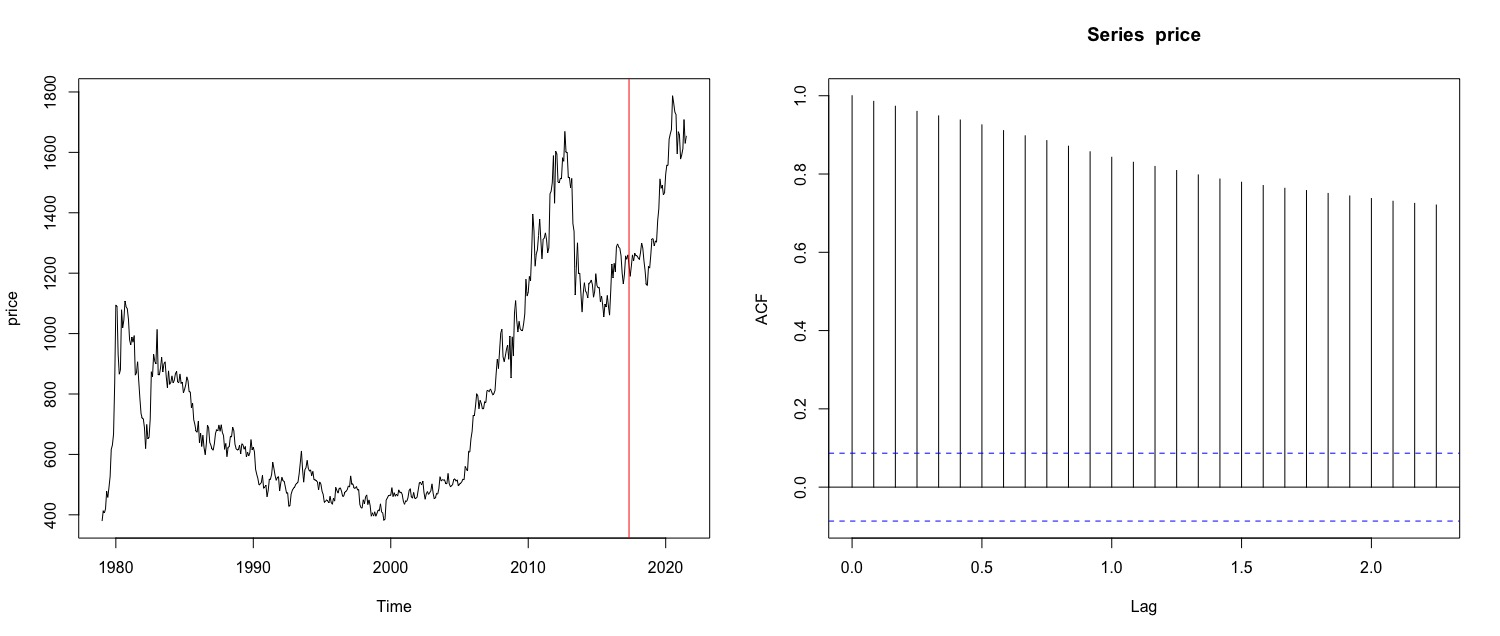
\includegraphics[width=\linewidth]{Image/intro-plot.jpeg}
    \caption{Time Series plot and ACF plot}
    \label{fig:intro-plots}
\end{figure}

Table \ref{table:head} is the first 5 rows of our time-series data. We remove the date component from the first column and create a time series object by month. We want to fit a forecasting model on the data and predict the next 2 years' monthly gold price. From figure \ref{fig:intro-plots}, we can see that our data has trend but no seasonality, since the ACF plot has a slow decay but not signs of periodic patterns or slow decay on seasonal lag. We also used classic decomposition on the data and observe significant trend and insignificant seasonality (see figure \ref{fig:decom-add} and figure \ref{fig:decom-mult} for details).

Additionally, we didn't observe any non-constant variance in the plot. For academic rigour, we performed the Fligner-Killeen test on the data set and extremely small p-value has been observe, implicating that non-constant variance exists in our data-set. However, when we try to use power transformation and Box-Cox method to remove the non-constant variance, neither method is helpful (see Appendix \ref{app:variance} for the result of F-test). 
Hence, we decide to move forward to try to fit models, but note that the results might not be valid since the data is non-stationary.


\subsection{Modelling}

We split the data-set into a training set and a test set, and use the test set MSE to select the best model within each category. 
The 90\% training set is from 1979-01 to 2017-03, and the 10\% test set is from 2017-04 to 2021-06 (see the red line in figure \ref{fig:intro-plots}).
Our goal is to predict the future 30 months of the gold price (up until 2023-12).

Three different types of models were applied to our data-set: regression (polynomial and Shrinkage methods), smoothing methods (exponential smoothing and Holt-Winters), and Box-Jenkins models (ARMA, ARIMA/SARIMA, etc).

\subsubsection{Regression}
\label{sec:regression}

We fit the polynomial regression with degree 2 to 10 on the training set and apply the model on the test set to predict. We then calculate the MSE and compare them across different degrees. The result and corresponding plot is shown in figure \ref{fig:reg_test_mse} and table \ref{tab:reg_test_mse}. 
Degree 2 has the smallest test set MSE. However, we know that our data is pretty complex looking at figure \ref{fig:intro-plots}, and whether a polynomial with only degree 2 can be a good fit remains questionable. The reason why our higher degree polynomial works terribly on the test set is due to bias-variance trade off (see appendix \ref{app:poly_summary} for details). 

Then, we fitted shrinkage methods on the training data to see if they do better than the polynomial regression. We used 10-fold cross validation to find the best $\lambda$ value. 

We find that
\begin{itemize}
    \item the best ridge model is at degree 9 with $\lambda=1.0000$
    \item the best lasso model is at degree 10 with $\lambda=0.2231$
    \item the best elastic model is at degree 9 with $\lambda=0.0302$
\end{itemize}
The detailed results refers to appendix \ref{app:shrinkage-summary}.

\begin{figure}[ht]
    \centering
    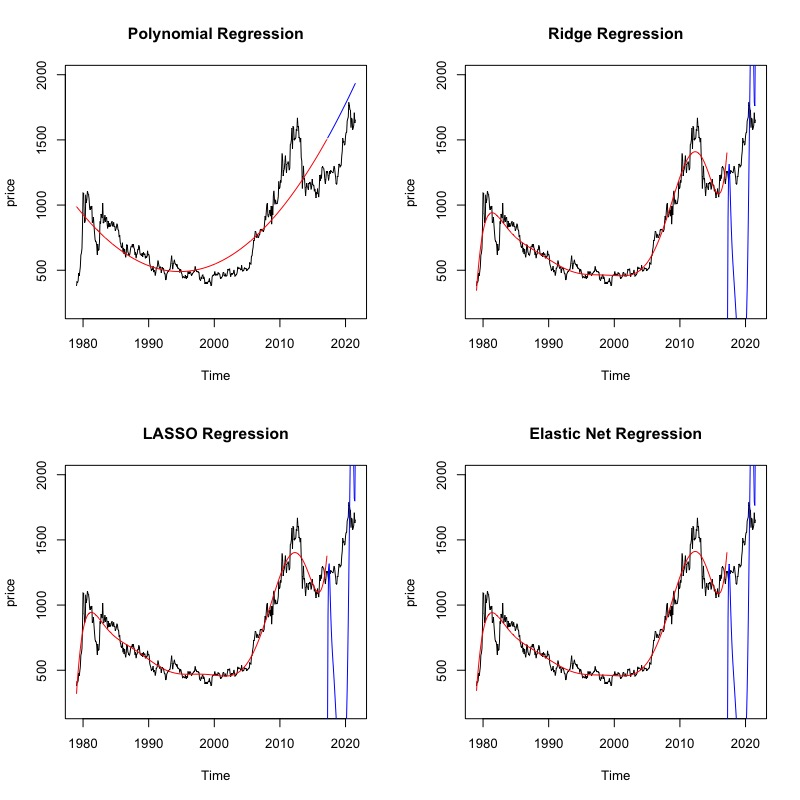
\includegraphics[width=0.75\linewidth]{Image/reg-summary.jpeg}
    \caption{Regressions Training vs. Test set}
    \label{fig:reg-summary}
\end{figure}

With the chosen degree and $\lambda$, we compared the prediction power of the four proposed models (polynomial, ridge, LASSO, and elastic net) with $\mathrm{MSE}_{pred}$ on the test set. 

\begin{table}[ht]
    \centering
    \begin{tabular}{|c|c|c|c|}
    \hline
    polynomial &  ridge  & lasso & elastic \\
    \hline\hline
    95478.66 & 1108226 & 1109892  & 1112580 \\
    \hline
    \end{tabular}
    \caption{Regression Prediction MSE}
\end{table}

It's clear that the polynomial regression with degree of 2 has the smallest $\mathrm{MSE}_{pred}$. 
We observed that this was an example of bias-variance trade off, since the polynomial regression had the worst fit, and all of the shrinkage methods had pretty descent fit. The high bias brought low variance in prediction, thus the polynomial regression surprisingly had a much better prediction on the test set than any of the shrinkage methods.

Hence, we chose it as our best regression model and moved on to see how it fitted on the entire data-set, and whether the model assumptions would be met.

Now, we fitted the optimal polynomial regression on the entire data-set (see Appendix \ref{app:poly_summary} for summary of the model) and calculated its residual of the whole data set. We also performed a model diagnostic to check whether the residuals follows the model assumptions.

\begin{figure}[ht]
    \centering
    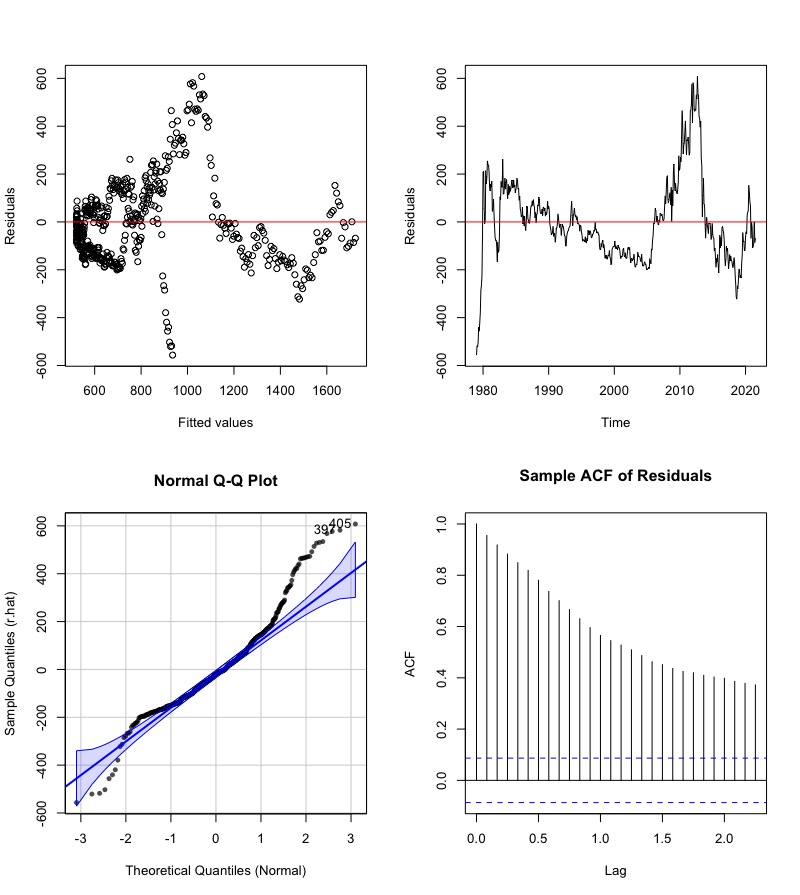
\includegraphics[width=0.6\linewidth]{Image/poly-res-diagnostic.jpeg}
    \caption{Polynomial Regression Residual Diagnostics}
    \label{fig:poly-res-diag}
\end{figure}

From figure \ref{fig:poly-res-diag}, we could see that the residuals 
\begin{itemize}
    \item did'nt have constant mean: trend was observed in the residuals plot,
    \item had correlation with the fitted values: trend was observed in the residuals vs. fitted values plot,
    \item was not normal: the Q-Q plot had a significant amount of data points falling out of the confidence interval,
    \item was correlated with each other: the ACF plot had very significant lags and has exponential decay.
\end{itemize}


\subsubsection{Smoothing Methods}
\label{sec:smooth}

We performed single exponential smoothing, double exponential smoothing, additive and multiplicative Holt-Winters algorithm on the training set, and applied the model on the test set to see how strong the fit and prediction power is. 
The model selection criteria was $\mathrm{MSE}_{pred}$ as well.

\begin{figure}[ht]
    \centering
    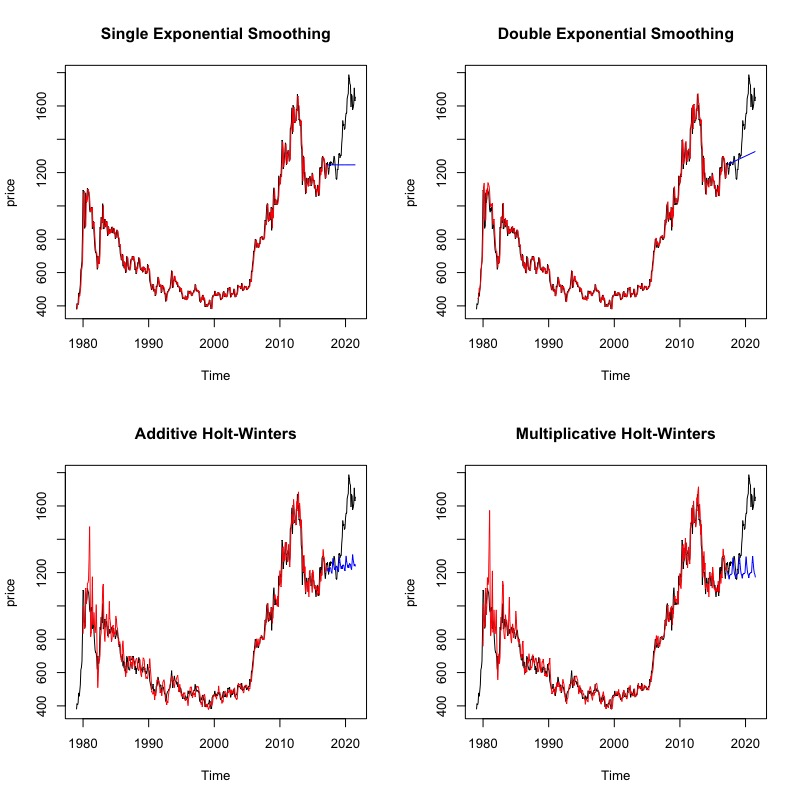
\includegraphics[width=0.75\linewidth]{Image/smoothing-summary.jpeg}
    \caption{Smoothing Methods Training vs. Test}
    \label{fig:smoothing-comp}
\end{figure}
\begin{table}[H]
    \centering
    \begin{tabular}{|c|c|c|c|}
    \hline
    single & double & additive HW & multiplicative HW \\
    \hline\hline
    68041.7 & 47731.91 &  67930.53  &  83083.73 \\
    \hline
    \end{tabular}
    \caption{Smoothing Methods Prediction MSE}
\end{table}

From the R output, the smallest MSE resulted in the double exponential smoothing. By figure \ref{fig:smoothing-comp}, we could see that even the model is almost perfect fit, the prediction for the test set was quite terrible. 
We concluded it as an extreme example of bad bias-variance trade-off. Obviously, smoothing methods were not good choices for predicting the trend of the gold price.


To check the model assumption, we used the same four plots as in the regression section \ref{sec:regression}.

\begin{figure}[H]
    \centering
    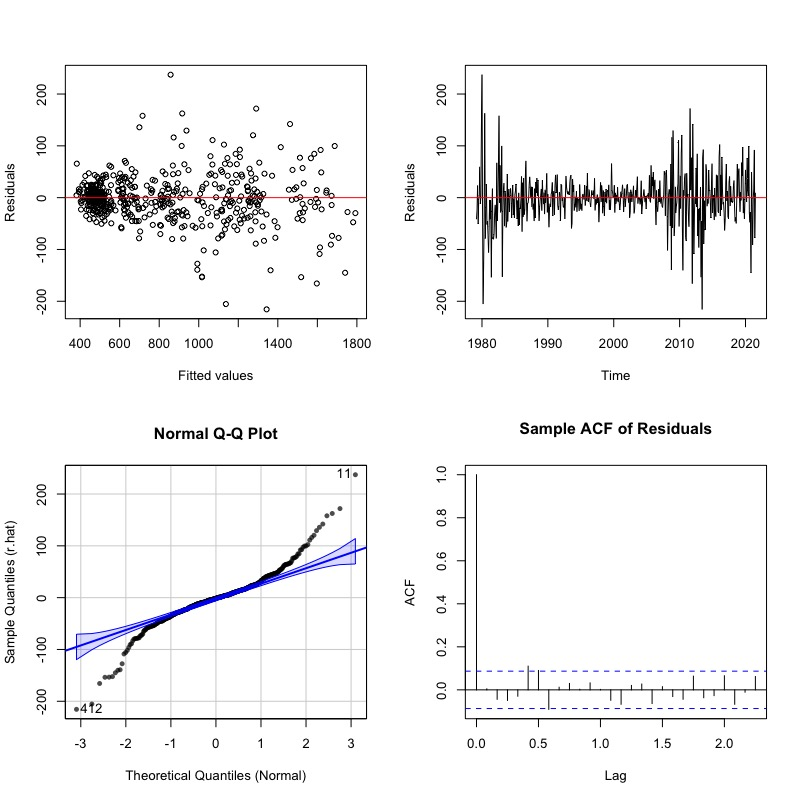
\includegraphics[width=0.6\linewidth]{Image/smooth-res.jpeg}
    \caption{Double Exponential Smoothing Residual Diagnostics}
    \label{fig:des-res-diag}
\end{figure}

Figure \ref{fig:des-res-diag} showed that the residuals
\begin{itemize}
    \item were not correlated with the fitted values
    \item had constant mean of 0, as seen in the residual plot. However, this plot also showed the non-constant variance in the residuals. This was due to the overall non-constant variance issues we'd discussed earlier (\ref{app:variance}),
    \item were not normal, which might be influenced by the non-constant variance,
    \item had no trend or seasonality, as illustrated in the sample ACF plot.
\end{itemize}


Therefore, the only source of non-stationarity was the non-constant variance. 


\subsubsection{Box-Jenkins Models}
\label{sec:boxjenkins}

From figure \ref{fig:intro-plots}, we saw that the data contains significant trend and no seasonality. Hence, we performed regular differencing to first remove non-stationarity from the data.

\begin{figure}[ht]
    \centering
    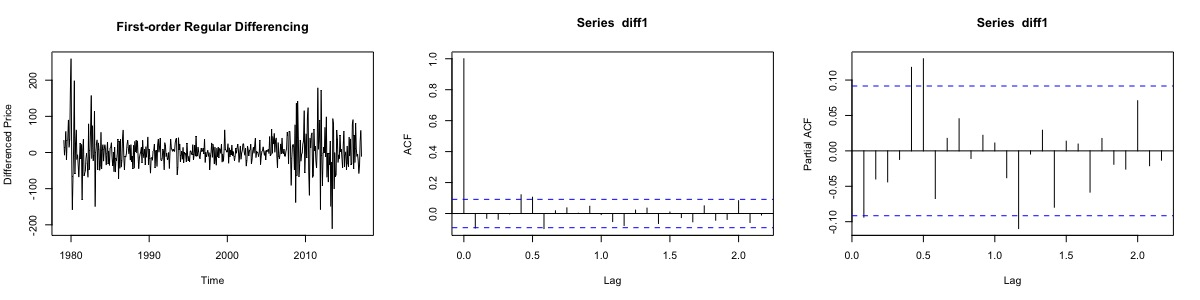
\includegraphics[width=\linewidth]{Image/diff1.jpeg}
    \caption{First order Regular Differencing}
    \label{fig:diff1}
\end{figure}

After performing one regular differencing on the data, the trend seemed to be removed from the data since there was no linear decay in the ACF plot. To be sure that no more differencing was needed, we performed another differencing, and figure \ref{fig:diff2} confirmed this conclusion. To avoid over-differencing, we stopped here and moved on to propose models.

Based on the ACF and PACF plot (\ref{fig:diff1}), we proposed several ARIMA models with no seasonality:
\begin{description}
    \item [ARIMA(0,1,1)] We observed that the ACF plot cuts off after lag 1, and the PACF plot had a damped sine wave. The spikes in the ACF plot after lag 1 was due to the 95\% confidence interval.
    \item [ARIMA(1,1,0)] We observed that the ACF plot has a damped sine wave, and the PACF plot cut off after lag 1 (we can see a little spike on lag 1). The spikes in the PACF plot after lag 1 was due to the 95\% confidence interval.
    \item [ARIMA(0,1,5)] We observed that the ACF plot cut off after lag 5, and the PACF plot had a damped sine wave. The spikes in the ACF plot after lag 5 was due to the 95\% confidence interval.
    \item [ARIMA(0,1,6)] We observed that the ACF plot cut off after lag 6, and the PACF plot had a damped sine wave. The spikes in the ACF plot after lag 6 was due to the 95\% confidence interval.
    \item [ARIMA(6,1,0)] We observed that the ACF plot had a damped sine wave, and the PACF plot cut off after lag 6. The spike in the PACF plot after lag 6 was due to the 95\% confidence interval.
    \item [ARIMA(1,1,1)] As above, we observed damped sine wave in both ACF and PACF plots.
    \item [ARIMA(p,1,q)] We can also tried other ARMA methods with larger $p$ and $q$ values.
\end{description}


\begin{table}[ht]
    \centering
    \begin{tabular}{|c|c|c|c|c|}
     \hline
      Model  &  $\mathrm{MSE}_{pred}$ &  AIC &  AICc &   BIC \\
      \hline\hline
ARIMA(0,1,1)& 43795.86& 10.48568& 10.48573& \textbf{10.51271} \\
ARIMA(1,1,0)& \textbf{43692.13}& 10.48642& 10.48648& 10.51345 \\
ARIMA(0,1,5)& 46688.48& 10.47991& 10.48032& 10.54299 \\
ARIMA(0,1,6)& 49255.66& 10.47709& 10.47764& 10.54918 \\
ARIMA(6,1,0)& 47231.58& \textbf{10.47324}& \textbf{10.47378}& 10.54532 \\
ARIMA(1,1,1)& 44388.76& 10.48873& 10.48884& 10.52477 \\
ARIMA(1,1,2)& 44479.14& 10.49295& 10.49314& 10.53800 \\
ARIMA(2,1,1)& 44517.89& 10.49288& 10.49308& 10.53794 \\
ARIMA(2,1,2)& 44396.06& 10.49741& 10.49770& 10.55148 \\
\hline
    \end{tabular}
    \caption{Box-Jenkins Methods Comparison}
    \label{tab:bj_comp}
\end{table}
\begin{figure}[ht]
    \centering
    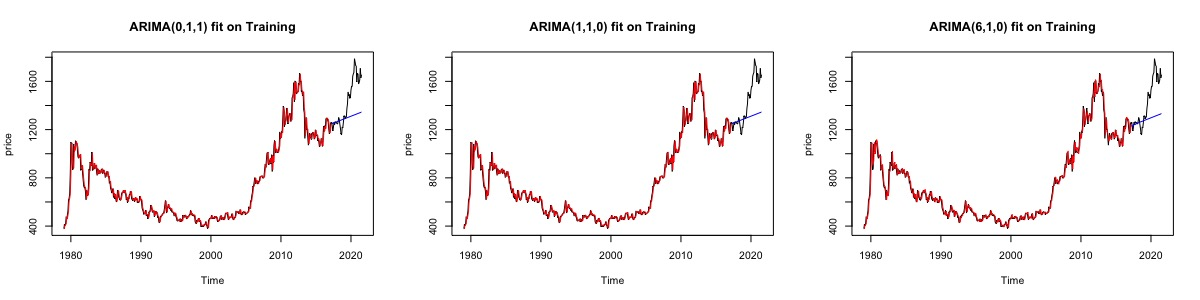
\includegraphics[width=\linewidth]{Image/arima-fit-comp.jpeg}
    \caption{ARIMA models fit on Training set}
    \label{fig:arima-fit-train}
\end{figure}

After calculating the MSE, AIC, AICc and BIC, which are shown in table \ref{tab:bj_comp}, we found that ARIMA(6,1,0), ARIMA(0,1,1), and ARIMA(1,1,0) all had better prediction power than the rest proposed models. We included the later two here because ARIMA(6,1,0) had 6 parameters comparing to the other two, and we tried to avoid choosing a model with too many parameters.
Looking at figure \ref{fig:arima-fit-train}, we saw that all three models have similar fit and prediction, so we would perform residual analysis on all three models to find the best model.

\begin{minipage}{\textwidth}
  \begin{minipage}[b]{0.49\textwidth}
    \centering
    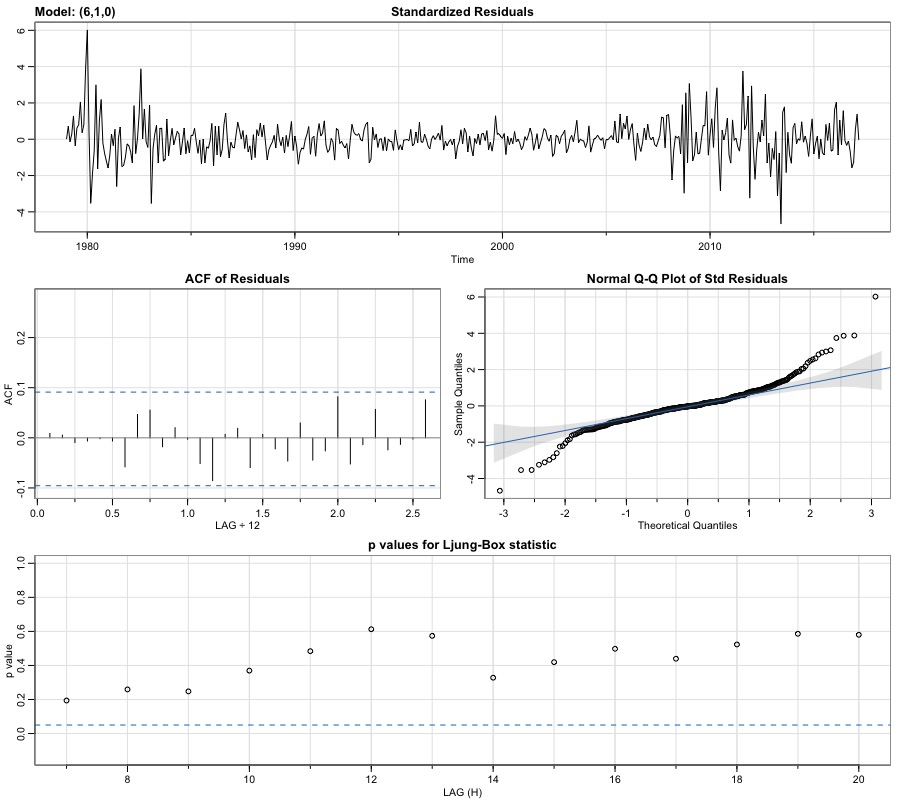
\includegraphics[width=\linewidth]{Image/bj610.jpeg}
    \captionof{figure}{ARIMA(6,1,0) on Training set}
    \label{fig:arima610}
  \end{minipage}
  \hfill
  \begin{minipage}[b]{0.49\textwidth}
    \centering
    \centering
    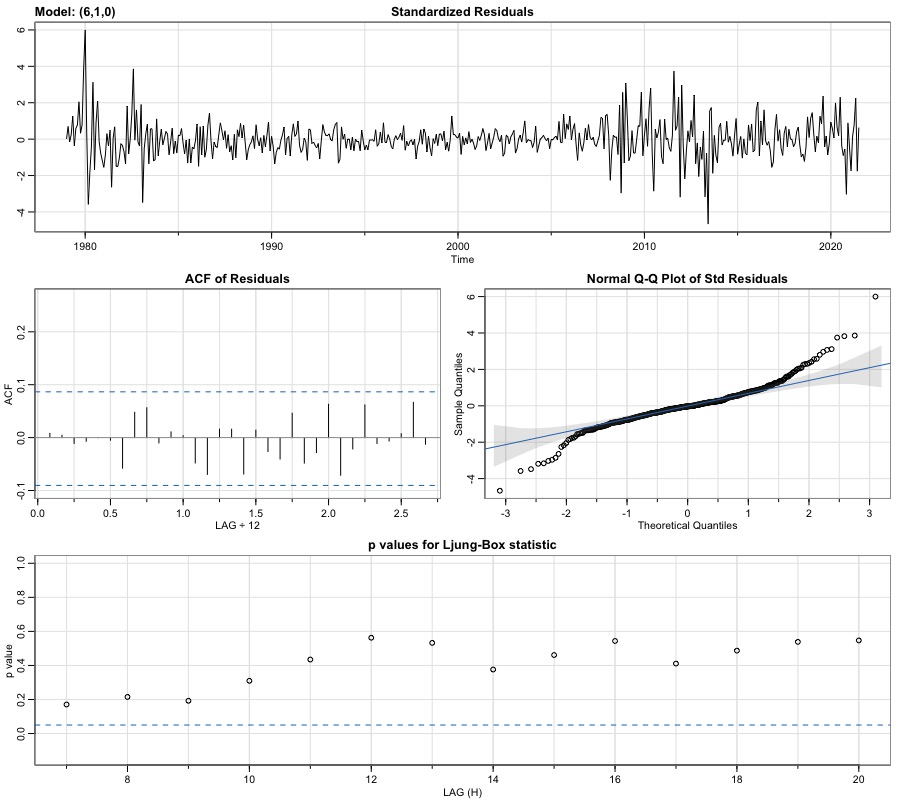
\includegraphics[width=\linewidth]{Image/fianl-arima.jpeg}
    \captionof{figure}{Final ARIMA Model Residual Analysis}
    \label{fig:arima_res}
  \end{minipage}
\end{minipage}

In Figure \ref{fig:arima610}, we could see that the residuals have constant mean, no seasonality, not normal (might due to the variance issue \ref{app:variance}), and the p values seemed great. Other than non-constant variance, the residuals were pretty much stationary. 
We also included the residual analysis for ARIMA(1,1,0) (figure \ref{fig:arima110}) and ARIMA(0,1,1) (figure \ref{fig:arima011}) in Appendix, and they didn't look as good as this model.

After checking the assumptions, we fitted the model on the entire data-set and estimate the parameters. 

\begin{table}[ht]
    \centering
    \begin{tabular}{|c|c|c|c|c|}
     \hline
      Model  &  $\mathrm{MSE}$ &  AIC &  AICc &   BIC \\
      \hline\hline
      ARIMA(6,1,0) & 2012.242 & 10.47854 & 10.47897 & 10.54496 \\
    \hline
    \end{tabular}
    \captionof{table}{Final ARIMA Fit and Prediction Power}
    \label{tab:arima_fit_pred}
\end{table}

We could see that the residuals (figure \ref{fig:arima_res}) matched the model assumptions, except non-constant variance and deviance in normality.




\vspace{1cm}
\begin{center}
    \noindent\rule{10cm}{0.4pt}
\end{center}


\section{Conclusions}

\subsection{Statistical Conclusions}

We used the following criteria to compare the selected regression, smoothing, and Box-Jenkins model:
\begin{enumerate}
    \item $\mathrm{MSE}_{pred}$ on the testing set
    \item $\mathrm{MSE}$ on the entire data-set
    \item Residual analysis
\end{enumerate}
The first analyzed the prediction power of the model; the second analyzed the fit of the model, and the third showed the validity of the model.

\begin{table}[H]
    \centering
    \begin{tabular}{|c|c|c|}
    \hline
     Model &  $\mathrm{MSE}_{fit}$ & $\mathrm{MSE}_{pred}$ \\
     \hline\hline
     Polynomial & 30239.665 &  95478.66 \\
    Smoothing &  2124.056&  47731.91 \\
    Box-Jenkins &  \textbf{2012.242}  & \textbf{47231.58} \\
    \hline
    \end{tabular}
    \caption{Final Comparison between 3 models}
\end{table}

The above table shows that the Box-Jenkins model (\ref{sec:boxjenkins}) had strongest fit and prediction power among all three. And if we look back at the residual analysis of the 3 models (figure \ref{fig:poly-res-diag}, figure \ref{fig:des-res-diag}, figure \ref{fig:arima_res}), the ARIMA model's residuals are the closest to the model assumption. Therefore, we conclude that ARIMA(6,1,0) is the best model to predict the monthly gold price data we have.

Now, we would use ARIMA(6,1,0) to predict the next 30 months' gold price.

\begin{figure}[H]
    \centering
    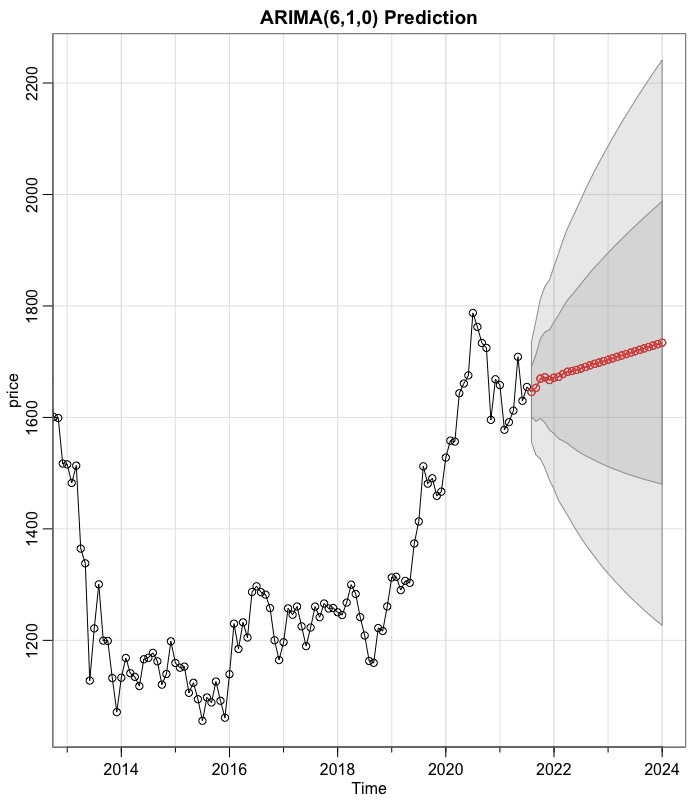
\includegraphics[width=0.5\linewidth]{Image/arima-pred.jpeg}
    \caption{ARIMA(6,1,0) Prediction}
    \label{fig:arima-pred}
\end{figure}
\begin{table}[H]
    \centering
    {\scriptsize
    \begin{tabular}{|c|c|c|c|c|c|c|c|c|c|c|c|c|}
    \hline
year & Jan & Feb & Mar & Apr & May & Jun & Jul & Aug & Sep & Oct & Nov & Dec \\
\hline\hline
2021 & & & & & & & & 1645.730 & 1653.005 & 1669.634 & 1672.018 & 1667.086 \\
\hline
2022 & 1671.276 & 1672.802 & 1677.870 & 1681.929 & 1683.312 & 1685.172 & 1687.807 & 1690.540 & 1693.578 & 1696.108 & 1698.402 & 1700.877 \\
\hline
2023 & 1703.453 & 1706.077 & 1708.667 & 1711.164 & 1713.662 & 1716.197 & 1718.749 & 1721.302 & 1723.837 & 1726.362 & 1728.893 & 1731.431 \\
\hline
    \end{tabular}
    }
    \caption{ARIMA(6,1,0) Prediction values}
\end{table}

However, due to the non-constant variance within the residuals, the validity of the prediction interval remained questionable.

\subsection{Connect to the Context}

In this project, we found that the gold price was pretty much hard to predict using a time-series model due to the complexity and cluster variation existing within this topic. The price is not only tied to time but also many other factors. As mentioned in the introduction, some research has already put effort in this prediction and include parameters such as NASDAQ index, which relates to data from the stock market.

As a result, there were several change points in the data-set, e.g. around the 1980s, 2010s, and 2020s. We could guess that the first is due to the stock market recession in 1980-1981, the second is due to the financial crisis in 2007-2008, and the last is due to the COVID-19 pandemic. All these global incidents cause the high variation and non-predictable pattern in the data-set, which is another reason why it's hard to remove the non-constant variance (\ref{app:variance}).

Our predictions above are the monthly gold prices from 2021 August to 2023 December. The monthly gold price would have a steady and slowly increasing trend, but the variation in our results exists and was pretty huge as shown.






\clearpage
\appendix
\section{Additional Figures}
\begin{figure}[H]
    \centering
    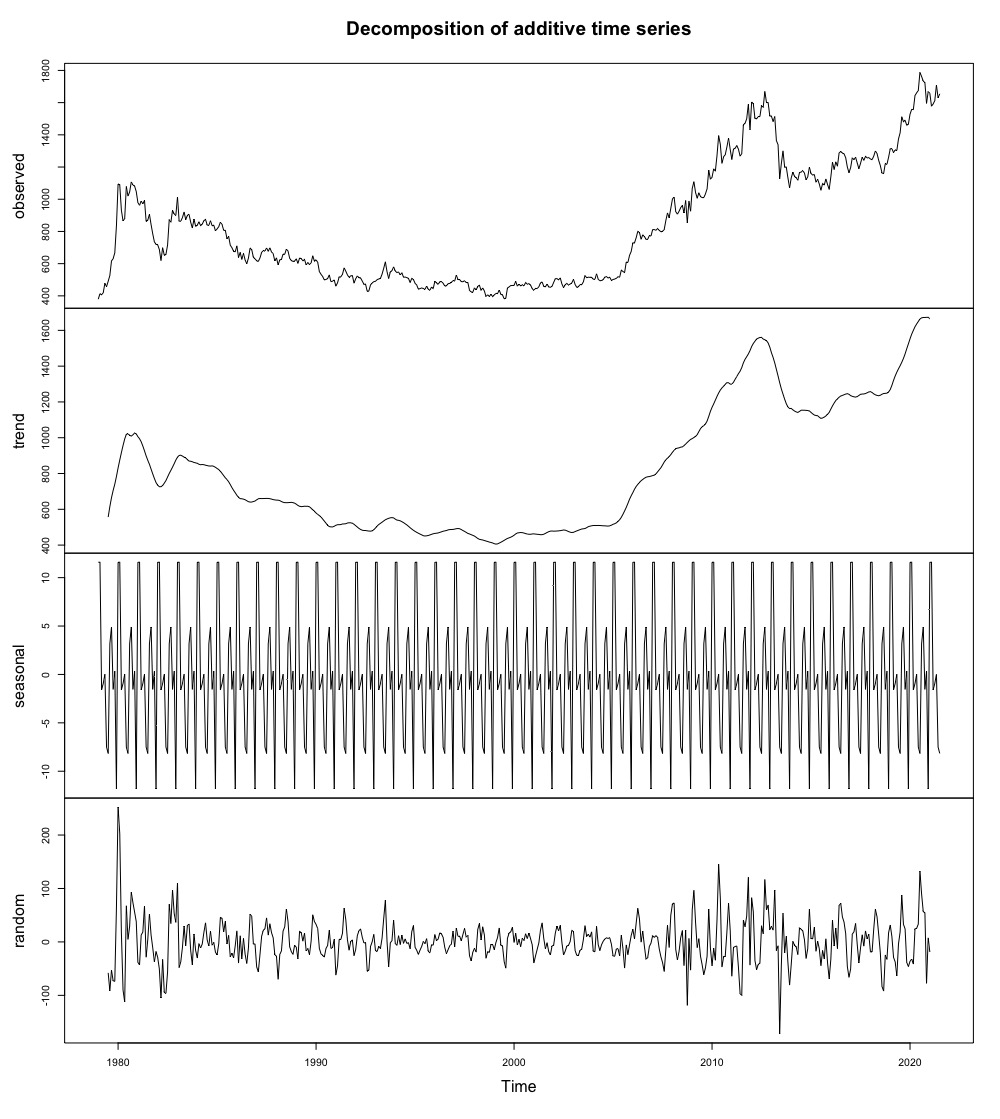
\includegraphics[width=0.75\linewidth]{Image/decompse-add.jpeg}
    \caption{Additive decomposition plot}
    \label{fig:decom-add}
\end{figure}
\begin{figure}[H]
    \centering
    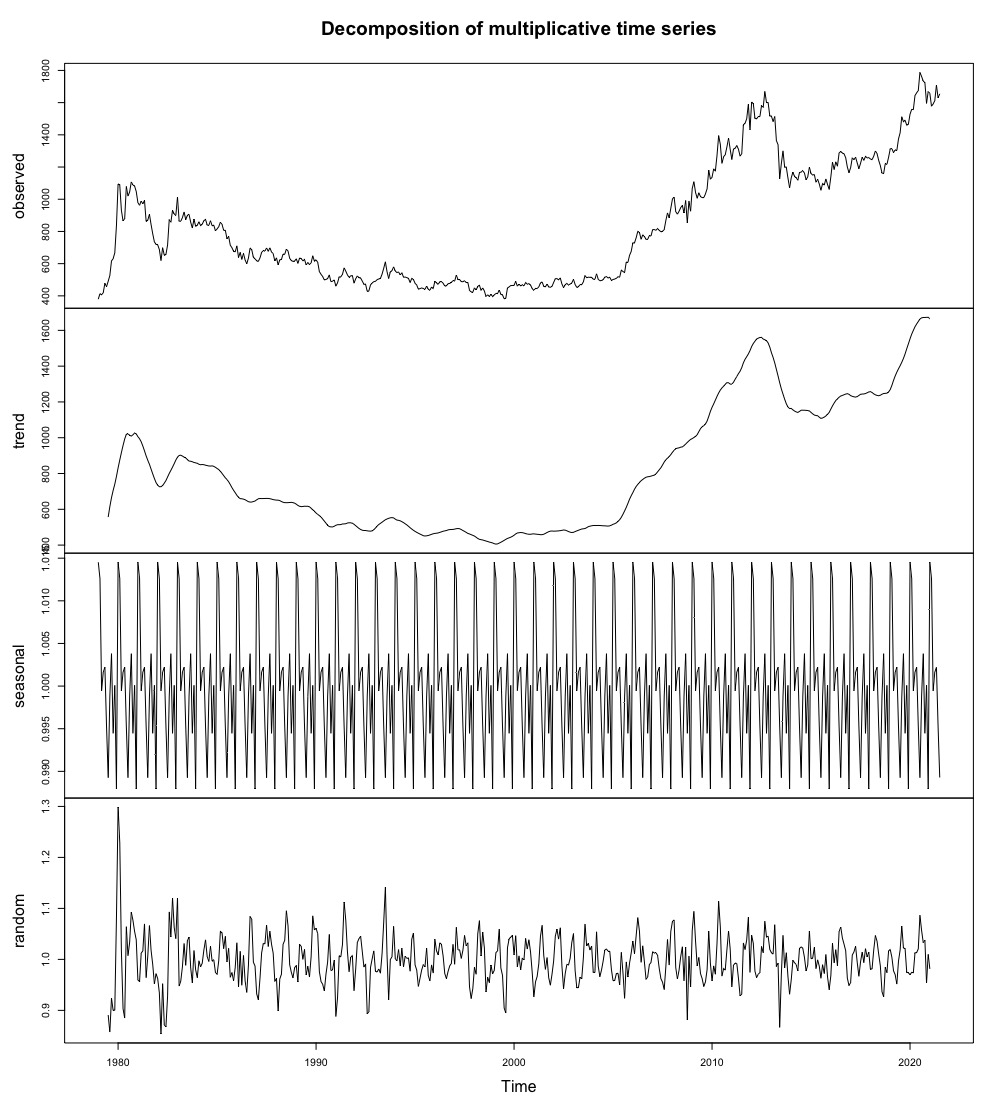
\includegraphics[width=0.75\linewidth]{Image/decompose-mult.jpeg}
    \caption{Multiplicative decomposition plot}
    \label{fig:decom-mult}
\end{figure}


\section{Supplementary Material}

\subsection{Non-constant Variance}
\label{app:variance}

We got the following when performing the Fligner test on the entire data:
\begin{lstlisting}
Fligner-Killeen test of homogeneity of variances
data:  price and seg
Fligner-Killeen:med chi-squared = 197.01, df = 4, p-value < 2.2e-16
\end{lstlisting}
We want to choose $\alpha$ from $\{-2,-1.5,-1,-0.5,0,0.5,1.5,2\}$.
When we use the Boxcox method, we get the following graph:
\begin{figure}[H]
    \centering
    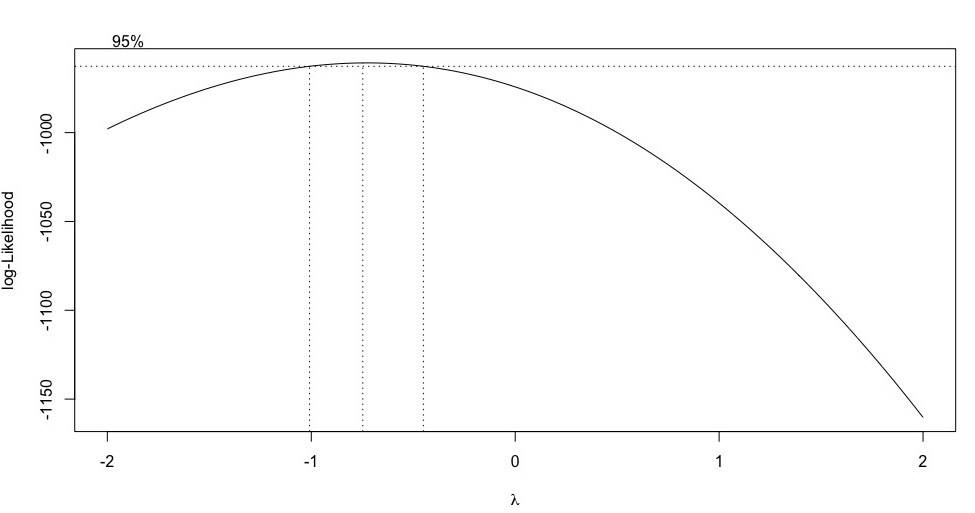
\includegraphics[width=0.5\linewidth]{Image/boxcox.jpeg}
    \caption{Boxcox result}
\end{figure}
When we again test on the power transformed data with $\alpha=-0.7474747$, we get
\begin{lstlisting}
Fligner-Killeen test of homogeneity of variances
data:  price^bx$x[which.max(bx$y)] and seg
Fligner-Killeen:med chi-squared = 107.15, df = 4, p-value < 2.2e-16
\end{lstlisting}
The extremely small p-value doesn't improve our results above.

We also compare the fligner test result on each $\alpha$ in the above list to find the optimal $\alpha$. The p-values from each test is as follows:
\begin{figure}[H]
    \centering
    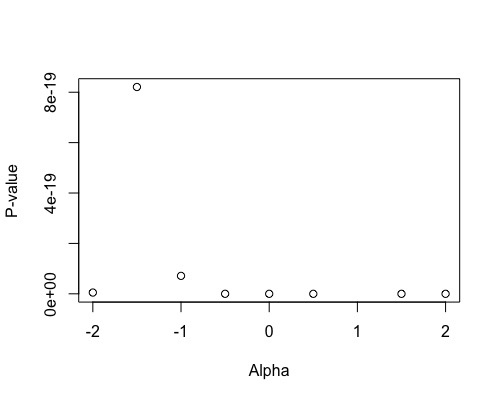
\includegraphics[width=0.5\linewidth]{Image/fligner-pval.jpeg}
    \caption{Fligner p-values}
\end{figure}
All the p values are extremely small, which means that any of $\alpha$ doesn't remove non-constant variance in our data.

\subsection{Polynomial Regression Model}
\label{app:poly_summary}

\textbf{Model selection results}:

\begin{minipage}{\textwidth}
  \begin{minipage}[b]{0.49\textwidth}
    \centering
    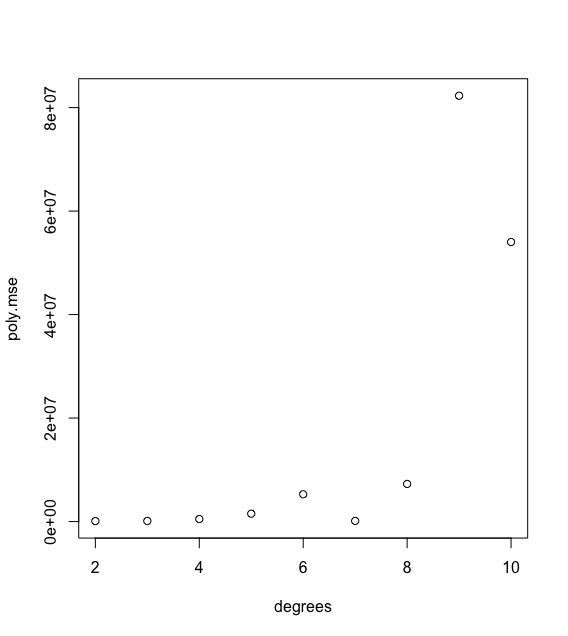
\includegraphics[width=0.75\linewidth]{Image/poly-test-mse.jpeg}
    \captionof{figure}{Polynomial regression test set MSE}
    \label{fig:reg_test_mse}
  \end{minipage}
  \hfill
  \begin{minipage}[b]{0.49\textwidth}
    \centering
    \begin{tabular}{|c|c|}
    \hline
    degree &  $\mathrm{MSE}_{pred}$ \\
    \hline\hline
    2  &  95478.66 \\
    3 & 116093.35 \\
    4 &  489939.41 \\
    5 & 1521066.09 \\
    6 & 5275901.68 \\
    7  & 120539.58 \\
    8 & 7270130.42 \\
    9 & 82291940.62 \\
    10 &  54021934.33 \\
    \hline
    \end{tabular}
    \captionof{table}{Polynomial regression test set MSE}
    \label{tab:reg_test_mse}
    \end{minipage}
\end{minipage}

We observed that higher polynomial degree result in a higher prediction MSE. This is because models with higher polynomial degree fits better on the training set (smaller bias) but consequently has a higher variance.

\begin{figure}[h]
    \centering
    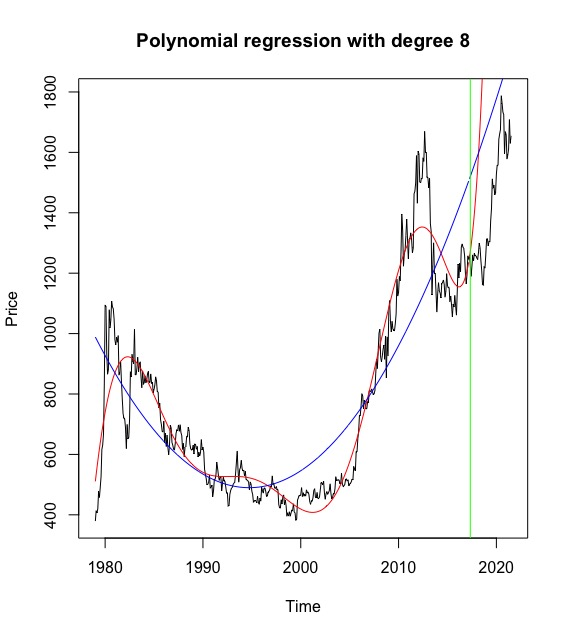
\includegraphics[width=0.5\linewidth]{Image/poly-comp.jpeg}
\end{figure}

The above plot shows the model with degree 8 (red) and degree 2 (blue). Degree 8 model fits the data much better than the degree 2 model, but it has a much worse prediction comparing to degree 2 model.



\subsection{Shrinkage methods}
\label{app:shrinkage-summary}

\begin{figure}[H]
    \centering
    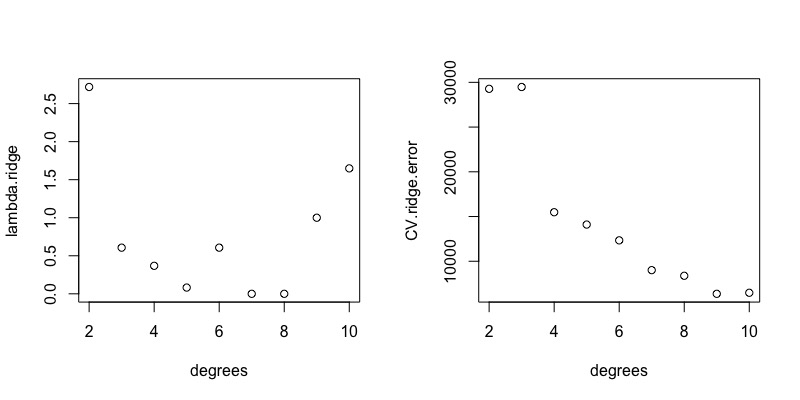
\includegraphics[width=0.75\linewidth]{Image/ridge-lambda.jpeg}
    \caption{Ridge Regression Lambda Values}

    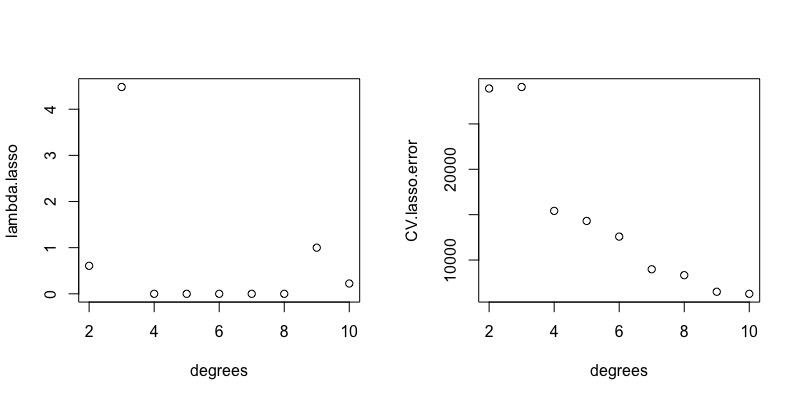
\includegraphics[width=0.75\linewidth]{Image/lasso-lambda.jpeg}
    \caption{LASSO Regression Lambda Values}

    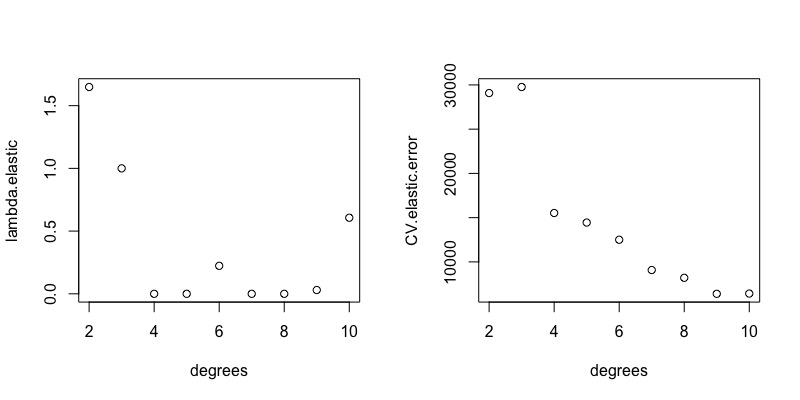
\includegraphics[width=0.75\linewidth]{Image/elastic-lambda.jpeg}
    \caption{Elastic Net Regression Lambda Values}
\end{figure}



\subsection{Box-Jenkins}

\textbf{Second-order regular differencing}:

\begin{figure}[ht]
    \centering
    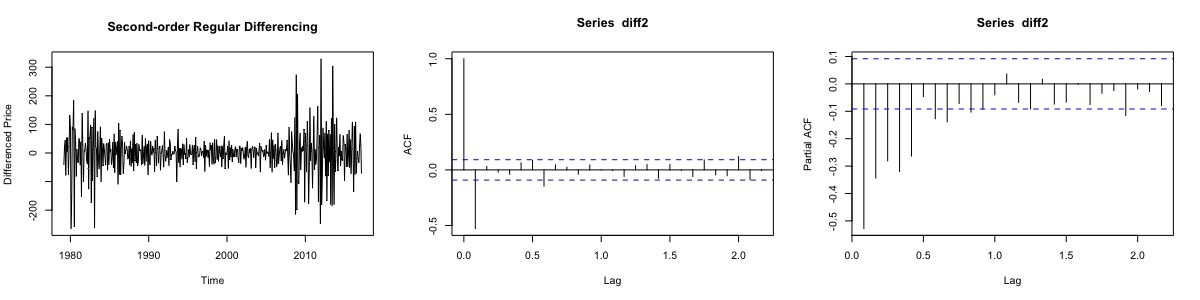
\includegraphics[width=\linewidth]{Image/diff2.jpeg}
    \caption{Second Regular Differencing}
    \label{fig:diff2}
\end{figure}

\textbf{Analysis for ARIMA(1,1,0) and ARIMA(0,1,1)}

\begin{minipage}{\textwidth}
  \begin{minipage}[b]{0.49\textwidth}
    \centering
    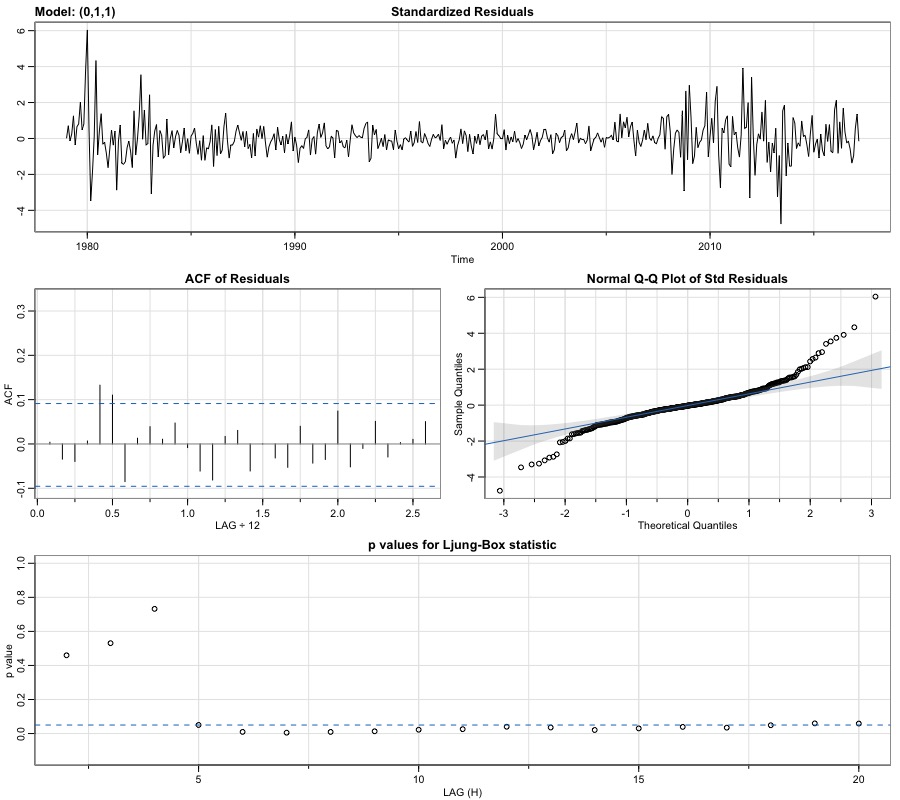
\includegraphics[width=\linewidth]{Image/bj011.jpeg}
    \captionof{figure}{ARIMA(0,1,1) on Training set}
    \label{fig:arima011}
  \end{minipage}
  \hfill
  \begin{minipage}[b]{0.49\textwidth}
    \centering
    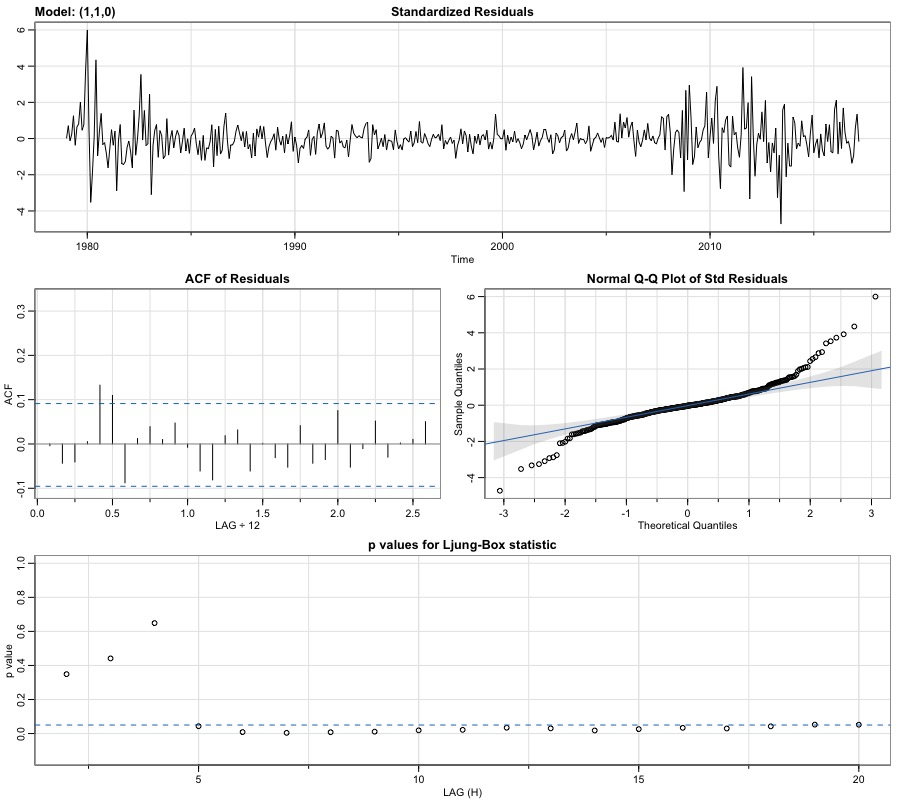
\includegraphics[width=\linewidth]{Image/bj110.jpeg}
    \captionof{figure}{ARIMA(1,1,0) on Training set}
    \label{fig:arima110}
  \end{minipage}
\end{minipage}



\newpage
\printbibliography
\end{document}
